\chapter{Tests and Results}
\label{tests}

In this chapter several experiments will be performed in order to assess the quality and features of technologies and developed application. The main goals are to obtain an empiric and realistic conclusion on which technology serves better the purpose of this thesis and to assess how the application fares when subject to different stress tests.

This chapter will be divided in two different sections: one regarding the comparison between Bluetooth and Wi-Fi Direct via different tests and other regarding the tests performed with the developed application, to better understand where it performs better and worse, proving or not if the theoretical choices made translate into actual performance gains.

\section{Bluetooth vs. Wi-Fi Direct}

This section will cover the differences, advantages and disadvantages of both Bluetooth and Wi-Fi Direct. A series of experiments will be conducted and their results analysed, providing a justification on which technology is best suited for this application and applications with a similar architecture and/or purpose.

Since the first implementation of Bluetooth in Android several releases have been developed. Different Bluetooth versions provide different \gls{QoS}, this may impact the performed tests as a device running a newer Bluetooth version may provide better results than a device running an older version. To avoid confusion all the tested devices will be running Bluetooth version 4.0.

The tests will range from battery consumptions to data rates analysis and most of them will be backed up by both theoretical and empirical results, although in some of them, due to the inability of getting precise measures, the results will be taken from previous developed works.

\subsection{Ranges of communication}

The ranges of communication of both technologies are of extreme importance. They can reduce or increase greatly the number of hops a packet has to pass through, in order to reach the destination. If the range of communication is too short, the number of connections made will increase, this may cause an overload of the network, and the deterioration of the communication medium. On the other hand, if the communication range is long the devices are able to jump through bigger hops, creating less traffic in the network and establishing the least possible number of connections.

Both technologies share some similarities, they are both dependent on the environment of the communication, the elements that are surrounding the devices and possible obstacles in the way. The experiments were conducted, for the obstacle experiment, in a corridor of Torre Norte in the vicinities of Instituto Superior Técnico and, for the line of sight experiment in the outside area of the same. It is important to note that although this experiments were made with as little interference as possible, there are certain elements that are impossible to controls, such as wireless communications from other devices, metal objects, such as metal lockers and cars.

Bluetooth establishes four different classes for the devices that may use this technology, depending on the transmitting power. Mobile phones are inserted in class 2 and, for that class, the specified average range of transmission in order to have a reliable connection is 10 meters, from \cite{bluetooth}.

Wi-Fi Direct on the other hand offers, theoretically, ranges of communication up to, approximately, 200 meters, from \cite{wfdrange}, which poses for a much better solution, in terms of network off-loading and general depth.

In order to verify these claims from both technologies, two mobile devices were taken to an open space, although with some limitations as described above, and several searches were made, until the devices stopped being discovered by one another. After measuring the distance between both devices, the results were taken, and prove what was already to be expected, although with some twists. 

Bluetooth was able to create a connection between devices from a distance up to 42 meters apart, see Figure \ref{fig:btMaxVisib} for the overall scheme of this experiment. This value is a lot more than what was expected judging by the theoretical value of 10 meters, although the health of the connection was not verified, see \ref{subsec:ftdr} for these tests. Using Wi-Fi Direct the devices were able to communicate from a maximum distance of 77 meters, see Figure \ref{fig:wfdMaxVisib} for the overall scheme of this experiment, which is, considerably, smaller than the theoretical value of 200 meters.

\begin{figure}[ht]
   \noindent\makebox[\textwidth]
    {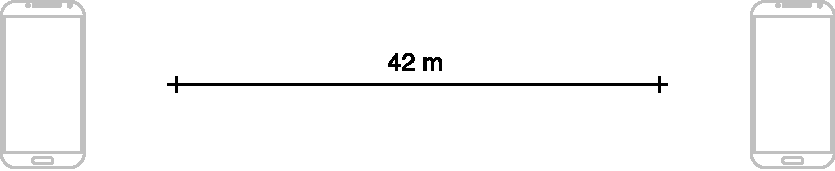
\includegraphics[width=0.8\textwidth]{images/bt_max_visib.pdf}}
	\caption{\label{fig:btMaxVisib} Max range of Bluetooth communication with line of sight between devices}
\end{figure}

\begin{figure}[ht]
   \noindent\makebox[\textwidth]
    {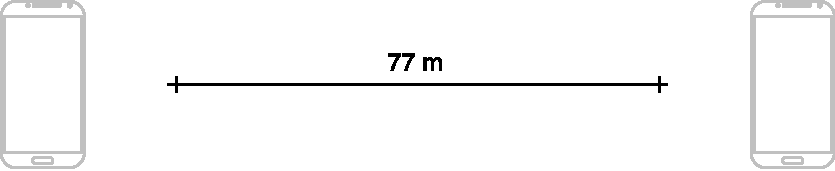
\includegraphics[width=0.8\textwidth]{images/wfd_max_visib.pdf}}
	\caption{\label{fig:wfdMaxVisib} Max range of Wi-Fi Direct communication with line of sight between devices}
\end{figure}

Both tests were made with a direct line of sight between devices. For the next ones there will be obstacles in the way of communication. It is expected that this affects greatly the communication ranges. The first test was made using Bluetooth technology where a wall was blocking the line of sight between devices, see Figure \ref{fig:btMaxInv}. The second test was made using Wi-Fi Direct, and, in order to maintain the same environment as the previous experiment, to get reliable results, it was situated in the same place as the first, see Figure \ref{fig:wfdMaxInv}. However, due to the environment configuration, it was impossible to recreate the experiment with only one wall, so two walls are now dividing the devices. Since the walls introduce a loss in the signal power, the more walls are between devices, the bigger the losses will be.

\begin{figure}[ht]
   \noindent\makebox[\textwidth]
    {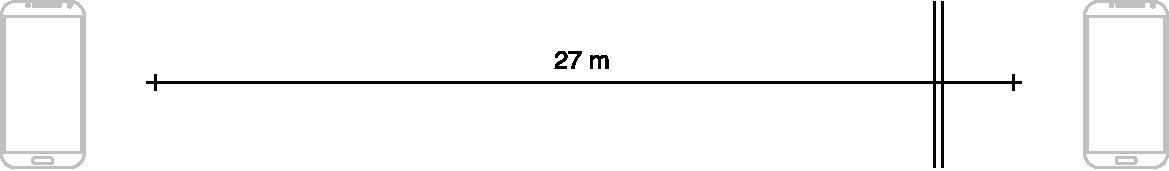
\includegraphics[width=0.8\textwidth]{images/bt_max_inv.pdf}}
	\caption{\label{fig:btMaxInv} Max range of Bluetooth communication without line of sight between devices}
\end{figure}

\begin{figure}[ht]
   \noindent\makebox[\textwidth]
    {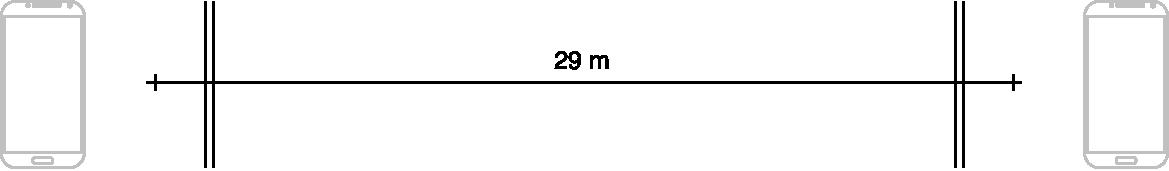
\includegraphics[width=0.8\textwidth]{images/wfd_max_inv.pdf}}
	\caption{\label{fig:wfdMaxInv} Max range of Wi-Fi Direct communication without line of sight between devices}
\end{figure}

As expected the obstacle, in this case the wall, created a significant decrease on the maximum range of communication. Bluetooth was able to communicate from a distance of 27m, closer to the theoretical 10 meters.

Wi-Fi Direct was also able to communicate from a smaller maximum distance, measuring 29 meters, with the signal passing through both walls. From a smaller distance it was verified that this technology could communicate with only wall in the way, meaning it also surpasses Bluetooth when an obstacle is in the way of communication.

After these experiments it is possible to conclude that Wi-Fi Direct is more desirable, since it provides better coverage than Bluetooth to similar areas. Also, there is no evidence that Wi-Fi Direct suffers more losses from obstacles, maintaining its desirability. This was already to expect, both from the theoretical values and from the transmission powers\footnote{Transmission powers impact directly the range of transmission, since they affect the signal strength, a crucial characteristic for receivers to better capture the transmissions. A bigger transmit power, usually, creates a bigger signal strength leading to the signal being capture over bigger distances, as referred in \cite{txpower}, for instance.}, since Bluetooth is mostly known for its lower transmit powers, if compared to technologies such as Wi-Fi.

\subsection{Battery consumptions}

\subsection{Discovery times}

The discovery times are a critical time factor for this application. The discovery process is the biggest time consumer during an application run thus, minimizing it comes with a great advantage for the overall performance of the application.

For this test three mobile devices where used: Samsung Grand Neo running Android version 4.2.2, Motorola Moto G2 running Android version 7.1 and Huawei P8 Lite running Android version 6.0, providing an heterogeneous sample space. For each device 10 discoveries where performed, providing a large sample size.

Bluetooth version 4.0 theoretically provides a discovery time of 10.24ms, as mentioned in \cite{btdisc1} and \cite{btdisc2}, and, to confirm this hypothesis, the three devices were put to the test. Each device was forced to do multiple discoveries with a different number of discovered devices, ranging from 0 devices found to 3 devices found.





\subsection{File transfer data rates}
\label{subsec:ftdr}

\section{Testing the developed application}

\subsection{Battery consumption during use}

\subsection{Discovery times}

\subsection{Connection times}

\subsection{File transfer data rates}




